\documentclass[conference]{IEEEtran}
\IEEEoverridecommandlockouts

% --- Пакеты для поддержки русского языка ---
\usepackage[utf8]{inputenc}
\usepackage[T2A]{fontenc}
\usepackage[russian]{babel}
% -------------------------------------------

\usepackage{cite}
\usepackage{amsmath,amssymb,amsfonts}
\usepackage{algorithmic}
\usepackage{graphicx}
\usepackage{textcomp}
\usepackage{xcolor}
\usepackage{caption}

\def\BibTeX{{\rm B\kern-.05em{\sc i\kern-.025em b}\kern-.08em
    T\kern-.1667em\lower.7ex\hbox{E}\kern-.125emX}}

\begin{document}

\title{Physics-Informed Neural Networks для моделирования динамики теплопроводности в 2D-пластине}

\author{\IEEEauthorblockN{1\textsuperscript{st} Янке Анастасия}
\IEEEauthorblockA{\textit{МИЭМ НИУ ВШЭ} \\
Москва, Россия \\
asianke@edu.hse.ru}
\and
\IEEEauthorblockN{2\textsuperscript{nd} Пырлицану Никита}
\IEEEauthorblockA{\textit{МИЭМ НИУ ВШЭ} \\
Москва, Россия \\
nepyrlitsanu@edu.hse.ru}
}

\maketitle

\begin{abstract}
    В данной работе рассматривается применение физически информированных нейронных сетей (Physics-Informed Neural Networks, PINN) для моделирования нестационарных процессов теплопроводности в двумерных структурах. В отличие от классических численных методов, требующих сложной генерации сеток, и стандартных подходов машинного обучения, зависящих от больших объемов размеченных данных, PINN интегрирует дифференциальные уравнения в частных производных (PDE) непосредственно в функцию потерь. Это позволяет нейронной сети обучаться соблюдению фундаментальных законов физики. В статье представлена подробная математическая постановка задачи, описана архитектура многослойного перцептрона с непрерывно дифференцируемыми функциями активации и предложен двухэтапный алгоритм оптимизации.
    \end{abstract}
    
    \begin{IEEEkeywords}
    Physics-Informed Neural Networks, PINN, теплопроводность, глубокое обучение, уравнение в частных производных, автоматическое дифференцирование.
    \end{IEEEkeywords}
    
    \section{Введение}
    
    Управление тепловыми режимами является критически важной задачей в современной инженерии: от проектирования систем охлаждения микропроцессоров до создания теплозащитных экранов в аэрокосмической отрасли. Проектирование систем охлаждения современных чипов требует высокоточного прогнозирования пространственно-временного распределения температур. Традиционное математическое описание этих процессов базируется на уравнении теплопроводности, решение которого в частных производных (PDE) критически важно для предотвращения локальных перегревов («hot spots»). Для предсказания распределения температур традиционно используются методы вычислительной гидродинамики и термодинамики (CFD), такие как метод конечных разностей (FDM) и метод конечных элементов (FEM). 
    
    Несмотря на высокую точность, классические подходы обладают рядом существенных недостатков. Во-первых, они требуют вычислительно затратной процедуры построения расчетных сеток, что в условиях высокой интеграции компонентов и сложности граничных условий приводит к экспоненциальному росту вычислительной стоимости («проклятие размерности»). Во-вторых, традиционные методы плохо адаптированы для работы в режиме реального времени и решения обратных задач (когда по известному температурному полю необходимо восстановить скрытые свойства системы). Это существенно ограничивает их применение в концепции цифровых двойников (Digital Twins).
    
    В последние годы парадигма научного машинного обучения (Scientific Machine Learning, SciML) предложила новый подход — физически информированные нейронные сети (PINN). Путем внедрения физических законов непосредственно в функцию потерь процесса обучения, исследователям удалось преодолеть зависимость от больших данных и создать бессеточные (mesh-free) алгоритмы аппроксимации дифференциальных уравнений. Данная статья посвящена подробному разбору теоретической и математической базы применения PINN для моделирования сложных тепловых процессов.
    
    \section{Обзор литературы}
    
    Концепция Physics-Informed Neural Networks была впервые формализована в 2019 году в прорывной работе Raissi, Perdikaris и Karniadakis \cite{raissi2019}. Авторы показали, что нейронные сети могут выступать в качестве универсальных аппроксиматоров решений уравнений в частных производных, если в качестве регуляризатора использовать невязку самого уравнения. Дальнейшее развитие и обобщение этого направления подробно описано в фундаментальном обзоре Karniadakis et al. \cite{karniadakis2021}.
    
    В области термодинамики применение PINN оказалось особенно успешным. Cai et al. \cite{cai2021} продемонстрировали высокую эффективность метода в задачах тепломассопереноса, показав возможность решения уравнений конвекции-диффузии. В работе Tamaddon-Jahromi et al. \cite{tamaddon2020} доказано, что PINN превосходят классические итеративные подходы при восстановлении скрытых граничных условий и свойств теплопроводности слоистых материалов. 
    
    Особое внимание в литературе уделяется микроэлектронике. He и Pathak \cite{he2020} предложили метод обучения без учителя (unsupervised learning) на базе автоэнкодеров для предсказания тепловых полей на микрочипах. Позднее Son et al. \cite{son2023} разработали модель PINN для терморегулирования микропроцессоров, позволяющую оценивать эффективность различных радиаторов. Более того, Benitez et al. \cite{benitez2024} доказали вычислительную легкость подобных моделей, успешно развернув физически-информированный цифровой двойник на базе микроконтроллера.
    
    Для работы с резкими градиентами температур применяются адаптивные функции активации \cite{jagtap2020}. Для глубокого понимания применимости PINN в задачах с разрывами и резкими скачками критически важны фундаментальные работы Mao et al. \cite{mao2020}, которые, исследуя гиперболические уравнения Эйлера, выявили значимость стратегического размещения сенсоров и влияния вычислительной точности на захват градиентов.
    
    Развитие PINN для гетерогенных сред и сложных доменов привело к созданию нейронных операторов. Важнейший вклад в эту область внесли Goswami et al. \cite{goswami2022}, предложив архитектуру физически-информированных глубоких нейронных операторных сетей (Physics-Informed DeepONet), которая объединяет аппроксимацию операторов с минимаксной оптимизацией функции потерь.
    
    \section{Базовые модели (Baselines) и постановка задачи}
    
    Для последовательного изучения возможностей физически-информированных нейронных сетей (PINN) в задачах термодинамики микроэлектроники были реализованы две базовые модели (baselines). Разработка велась с опорой на методологию, предложенную в работе Son et al. \cite{son2023}, с переходом от упрощенной абстрактной задачи к комплексной слоистой структуре.
    
    \subsection{Математическое описание тепловых процессов}
    Моделирование теплопереноса в твердотельных структурах основывается на фундаментальных принципах сохранения энергии. В то время как фундаментальные работы (например, Mao et al. \cite{mao2020}) фокусируются на гиперболических уравнениях Эйлера (сохранение массы, импульса и энергии), теплофизика микропроцессоров чаще оперирует параболическим уравнением теплопроводности. Однако при использовании активного жидкостного охлаждения в микроканалах необходимо учитывать адвективный член ($\mathbf{u} \cdot \nabla T$), что возвращает нас к сложности полной системы уравнений гидродинамики.
    
    Переход от феноменологического закона Фурье к PDE позволяет описать эволюцию температурного поля как функцию градиентов. Здесь прослеживается прямая аналогия с методом Шлирена (Schlieren photography), применяемым для визуализации градиентов плотности $\nabla \rho$ \cite{mao2020}. Подобно тому как методы PINN восстанавливают полные поля состояний из градиентных данных Шлирена, в теплофизике нейросеть может использовать данные инфракрасной термографии для выявления скрытых источников тепла.
    
    Для обеспечения единственности решения PDE обязательна строгая постановка условий Дирихле (на границе с хладагентом) и Неймана (на изолированных поверхностях). Вычислительная схема требует внедрения этих условий как мягких или жестких ограничений в функцию потерь. Сложность их реализации в классических сетках при неоднородной геометрии предопределяет целесообразность перехода к бессеточным (mesh-free) решателям.
    
    \subsection{Интеграция физики в архитектуру глубокого обучения}
    Концепция информированного обучения трансформирует нейросеть из статистического аппроксиматора в строгий вычислительный инструмент. Архитектура PINN минимизирует общую ошибку $\mathcal{L}$, состоящую из вклада данных и физической невязки:
    \begin{equation}
        \mathcal{L}(\theta) = MSE_{data} + MSE_{f}
    \end{equation}
    Критически важным аспектом является настройка весовых коэффициентов. Согласно исследованию Goswami et al. \cite{goswami2022}, вместо ручного подбора следует использовать процедуру минимаксной оптимизации самоадаптивных весов $\lambda$. Нейросеть минимизирует лосс по параметрам сети $\theta$ и одновременно максимизирует его по $\lambda$ (градиентный спуск по $\theta$ и восхождение по $\lambda$), фокусируя обучение на областях с наибольшей невязкой.
    
    Использование автоматического дифференцирования (AD) позволяет вычислять производные произвольного порядка без сеток, избавляя от проблем дискретизации FDM. Для обеспечения физичности решения (строгого соблюдения положительности абсолютной температуры в Кельвинах), к выходному слою сети применяется экспоненциальная функция активации.
    
    \subsection{Обзор многодоменных подходов и моделирование гетерогенных сред}
    Микропроцессорная система характеризуется экстремальной гетерогенностью: кремний, термоинтерфейсы (TIM) и медные радиаторы имеют разные коэффициенты проводимости. Для работы с такими системами PINN масштабируются до уровня нейронных операторов. Архитектура DeepONet \cite{goswami2022} реализует решение как тензорное произведение выходов двух сетей:
    \begin{equation}
        G_{\theta}(v)(\xi) = \sum_{k=1}^p \underbrace{br_k(v(s_1), \dots, v(s_m))}_{\text{Branch}} \cdot \underbrace{tr_k(\xi)}_{\text{Trunk}}
    \end{equation}
    Сеть ветвей (Branch net) кодирует входные функции (распределение мощностей), а сеть стволов (Trunk net) — пространственно-временные координаты. Это позволяет обучать оператор один раз для целого класса задач.
    
    На границах разделов сред необходимо выполнение условий непрерывности. При сложной геометрии применяются подходы gFNO+ и dgFNO+, использующие «bounding boxes» для отображения неструктурированной сетки на декартову решетку. Сравнительный анализ стабильности указывает на превосходство нелокальных ядерных сетей (NKN) над графовыми (GKN). NKN идентифицируют индекс итерационного слоя со схемой дискретизации по времени $\Delta t$, гарантируя положительную определенность оператора и исключая неустойчивость в глубоких слоях.
    
    \subsection{Вызовы, ограничения и обратные задачи}
    Одним из главных преимуществ PINN является эффективность в решении обратных задач. При идентификации коэффициента теплопроводности $\gamma$, как и в задачах Римана (Sod/Lax) у Mao et al. \cite{mao2020}, критическую роль играет стратегическое размещение сенсоров. Размещение единственного термодатчика ($T^*$) внутри подложки должно производиться в зоне активного изменения градиентов для обеспечения уникальности восстанавливаемого поля.
    
    Анализ сходимости (Mao et al., Section 4.1.4 \cite{mao2020}) доказывает, что использование одинарной точности (single precision) ведет к неудачам при захвате резких скачков. В микропроцессорах, где на границах материалов возникают экстремальные термические градиенты, использование двойной точности (double precision) является обязательным требованием.
    
    Несмотря на необходимость точной настройки гиперпараметров, гибридные архитектуры (подобные PI-DeepONet \cite{goswami2022}) открывают путь к созданию мощных адаптивных «цифровых двойников» процессоров нового поколения.
    

\subsection{Baseline 1: Однодоменная модель тепловыделения}

Первая базовая модель описывает распространение тепла в однородной изотропной 2D-пластине, которая концептуально представляет собой срез микрочипа. 

\section{Методология и этапы разработки модели}

Процесс разработки физически-информированной модели цифрового двойника был разделен на три этапа: верификация на основе классических решений, переход к нестационарным процессам и реализация многодоменной архитектуры.

\subsection{Этап 0: Верификация модели на основе уравнения Лапласа}

В качестве отправной точки и валидации предложенного подхода была выбрана задача реконструкции стационарного теплового поля, описанная в работе Benitez et al. (2025). В данной работе авторы используют сетку $5 \times 5$ узлов для мониторинга алюминиевой пластины, где значения в 12 граничных узлах задаются реальными датчиками-термисторами.

\textbf{Математическая постановка задачи референса.} Система описывается стационарным уравнением Лапласа:
\begin{equation}
    \Delta u = \frac{\partial^2 u}{\partial x^2} + \frac{\partial^2 u}{\partial y^2} = 0
\end{equation}
с граничными условиями Дирихле, задаваемыми вектором показаний датчиков $\mathbf{T}_{sensor}$.

\textbf{Алгоритм сравнения (Baseline Reference).} В статье-референсе для решения используется итерационный метод Либмана (модификация метода Якоби) с коэффициентом сверхрелаксации $\lambda = 1.5$ для ускорения сходимости:
\begin{equation}
    u_{i,j}^{(n+1)} = \frac{1}{4} \left( u_{i+1,j}^{(n)} + u_{i-1,j}^{(n)} + u_{i,j+1}^{(n)} + u_{i,j-1}^{(n)} \right)
\end{equation}

На данном этапе нами была обучена модель PINN, принимающая на вход только координаты $(x, y)$. Сравнение показало, что PINN успешно реконструирует внутренние значения температуры (в частности, в контрольной точке $T_{13}$ в центре пластины) с точностью, сопоставимой с методом конечных разностей, при этом обеспечивая непрерывность решения во всем домене. Однако, как отмечают сами авторы референса, данная модель ограничена стационарным режимом и не учитывает внутренние источники тепла.

\textbf{Архитектура и параметры обучения PINN.} Для решения задачи Лапласа была спроектирована полносвязная нейронная сеть (MLP) со следующими характеристиками:
\begin{itemize}
    \item \textbf{Входной слой:} 2 нейрона (координаты $x, y$).
    \item \textbf{Скрытые слои:} 6 последовательных слоев по 64 нейрона в каждом.
    \item \textbf{Функция активации:} гиперболический тангенс (Tanh), обеспечивающий необходимую гладкость вторых производных для вычисления оператора Лапласа.
    \item \textbf{Выходной слой:} 1 нейрон (реконструированная температура $T$).
\end{itemize}

Обучение проводилось в два этапа. На первом этапе использовался оптимизатор Adam (5000 эпох, скорость обучения $10^{-3}$) для быстрой минимизации глобальной ошибки. На втором этапе применялся алгоритм L-BFGS для прецизионной «подгонки» решения под граничные условия. Для стабилизации сходимости была применена нормализация целевой температуры в диапазон $[0, 1]$ и введено взвешивание функции потерь: $Loss_{total} = 1000 \cdot Loss_{BC} + 1 \cdot Loss_{PDE}$.

\textbf{Результаты и метрики.} В процессе обучения ошибка на границах ($Loss_{BC}$) снизилась с $4.14 \times 10^{-1}$ до $3.45 \times 10^{-5}$, что свидетельствует об очень точном соответствии модели «показаниям датчиков». Итоговое сравнение PINN с классическим методом конечных разностей (FDM) в контрольной точке $T_{13}$ (центр пластины) показало разницу всего в $0.406^\circ$C ($30.41^\circ$C у PINN против $30.00^\circ$C у FDM), что составляет менее 1\% от диапазона температур.

\begin{figure}[ht!]
    \centering
    
\includegraphics[width=0.5\textwidth]{C:/Users/nasty/local_projects/PZAD/pic/baseline0_compare_fdm_result.png}
    \caption{Сравнение дискретных температурных полей FDM и PINN в виде тепловых карт (сетка 5x5) и распределение абсолютной ошибки}
    \label{fig:heatmap_compare}
\end{figure}

\begin{figure}[ht!]
    \centering
    
\includegraphics[width=0.5\textwidth]{C:/Users/nasty/local_projects/PZAD/pic/baseline0_compare_fdm_result_2.png}
    \caption{Трехмерная визуализация температурных поверхностей (3D Surface) для численного решения и обученной нейросети}
    \label{fig:surface_compare}
\end{figure}

\begin{figure}[ht!]
    \centering
    
\includegraphics[width=0.5\textwidth]{C:/Users/nasty/local_projects/PZAD/pic/baseline0_compare_fdm_result5.png}
    \caption{Центральные профили распределения температуры: сравнение значений в узлах сетки по горизонтальному (y=0.5) и вертикальному (x=0.5) сечениям}
    \label{fig:profiles_compare}
\end{figure}

\textbf{Анализ графических результатов (рис. \ref{fig:baseline0_compare}).} Визуализация подтверждает высокую сходимость методов:
\begin{enumerate}
    \item \textbf{Тепловые карты (верхний ряд):} Демонстрируют идентичное распределение градиента от нагретой нижней грани ($60^\circ$C) к холодным краям ($20^\circ$C). Карта абсолютной ошибки фиксирует максимальные расхождения в зонах наиболее резкого изменения градиента, при этом ошибка не превышает $1.3^\circ$C.
    \item \textbf{3D-поверхности (средний ряд):} Наглядно показывают «форму» температурного поля. Поверхность PINN в точности повторяет геометрию FDM-решения, подтверждая отсутствие осцилляций и «галлюцинаций» нейросети внутри домена.
    \item \textbf{Линейные профили (нижний ряд):} Сечение по центру пластины при $y=0.5$ (горизонтальный срез) показывает симметричный куполообразный профиль, а срез при $x=0.5$ (вертикальный) — характерное нелинейное затухание температуры от источника к верхней грани. Практически полное наложение синей (FDM) и красной (PINN) линий верифицирует точность нейросетевого решателя.
\end{enumerate}
\subsection{Baseline 1: Нестационарная модель с источником тепла}

Для преодоления ограничений стационарной модели и обеспечения возможности мониторинга процессора в моменты пиковых нагрузок, постановка задачи была расширена. 

\textbf{Математическая постановка.} Распределение температуры $u(x, y, t)$ теперь подчиняется неоднородному уравнению теплопроводности, что позволяет учитывать тепловую инерцию материала и наличие активного источника энергии:
\begin{equation}
    \frac{\partial u}{\partial t} = \alpha \left( \frac{\partial^2 u}{\partial x^2} + \frac{\partial^2 u}{\partial y^2} \right) + Q(x,y)
    \label{eq:baseline1_pde}
\end{equation}
где $\alpha = 0.05$ — нормированный коэффициент температуропроводности. Функция $Q(x,y)$ моделирует тепловыделение процессорного ядра и задана в виде двумерного распределения Гаусса с центром в точке $(x_0, y_0) = (0.5, 0.5)$:
\begin{equation}
    Q(x,y) = Q_{max} \exp\left( -\frac{(x - x_0)^2 + (y - y_0)^2}{2\sigma^2} \right)
\end{equation}
Начальное условие (IC) задает однородную начальную температуру $u(x,y,0) = 20^\circ\text{C}$. Граничные условия (BC) выбраны холодными (условия Дирихле первого рода): на всех четырех границах квадрата постоянно поддерживается температура окружающей среды $20^\circ\text{C}$.

\textbf{Архитектура нейросети.} Для решения данной задачи применяется архитектура PINN, расширенная временной координатой на входе. Сеть представляет собой многослойный перцептрон (MLP), который принимает на вход кортеж $(x, y, t)$ и выдает скаляр температуры $\hat{u}_\theta(x, y, t)$. Архитектура состоит из 5 скрытых слоев по 60 нейронов. Для обеспечения возможности вычисления вторых пространственных производных используется функция активации $\tanh$.

\begin{figure}[ht!]
    \centering
    %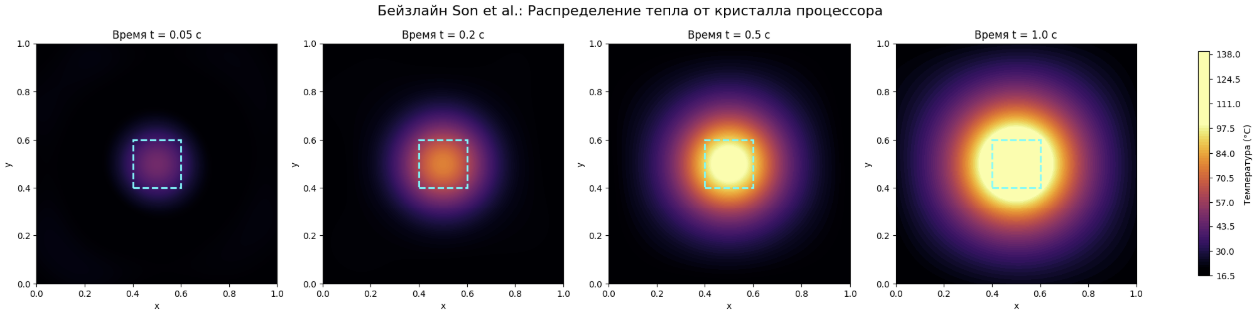
\includegraphics[width=0.5\textwidth]{pic/baseline1_result.png}
    \caption{Результат моделирования Baseline 1: динамика нагрева однородной пластины при включении центрального источника.}
    \label{fig:baseline1_res}
\end{figure}

\subsection{Baseline 2: Многодоменная модель со сложной структурой}

В реальных системах процессор не является однородным телом. Для повышения точности цифрового двойника вычислительный домен $\Omega$ был разделен на три подобласти с различными теплофизическими свойствами, имитирующими вертикальный разрез системы охлаждения:
\begin{itemize}
    \item $\Omega_1$ (\textbf{Chip}, $y \in [0, 0.2]$): Область генерации тепла с низким коэффициентом диффузии.
    \item $\Omega_2$ (\textbf{Heat Sink}, $y \in (0.2, 0.6]$): Медный или алюминиевый радиатор с высокой теплопроводностью.
    \item $\Omega_3$ (\textbf{Ambient}, $y \in (0.6, 1.0]$): Воздушная среда с низкой эффективностью передачи тепла.
\end{itemize}

Вместо одной нейросети используется ансамбль из трех независимых моделей $\hat{u}_1, \hat{u}_2, \hat{u}_3$. Для обеспечения физичности на выходе сетей применяется функция \texttt{Softplus}, гарантирующая положительность температуры.

Для корректной «сшивки» физических процессов на интерфейсах сред в функцию потерь вводится штраф за нарушение непрерывности температуры и теплового потока:
\begin{equation}
\begin{aligned}
    \mathcal{L}_{interface} = \sum_{j \in \{1,2\}} \left( \lambda_T \| \hat{u}_j - \hat{u}_{j+1} \|^2 + \right. \\
    \left. \lambda_q \left\| -k_j \frac{\partial \hat{u}_j}{\partial y} + k_{j+1} \frac{\partial \hat{u}_{j+1}}{\partial y} \right\|^2 \right)
\end{aligned}
\end{equation}
где $k_j$ — коэффициенты теплопроводности соответствующих слоев. Такой подход позволяет моделировать резкие изменения температурного градиента на границах материалов, что недоступно упрощенным моделям из референсной литературы.

\section{Результаты и обсуждение}
... (далее ваш текст про обучение, Adam/L-BFGS и анализ полей)    



\section{Data Processing and Reproducible Dataset}
In this project, PINN data include collocation points, boundary-condition points, and initial-condition points. The data-generation stage is moved into a dedicated module, \texttt{src/preprocessing.py}, to ensure reproducibility.

\textbf{Domain sampling.} Interior points are sampled via Latin Hypercube Sampling (LHS). Boundary points are generated separately for $x=0$, $x=1$, $y=0$, and $y=1$. Initial-condition samples are generated at $t=0$.

\textbf{Normalization.} Coordinates $(x,y,t)$ and temperature $T$ are min-max normalized to $[0,1]$. This stabilizes training and improves balance between different loss terms.

\textbf{FDM ground truth.} A classical finite-difference method (FDM) is used to generate reference temperature fields. The processed dataset is saved to \texttt{data/processed/pinn\_dataset.npz}, and normalization metadata is saved to \texttt{data/processed/pinn\_dataset\_meta.json}.

\section{Modeling and Experiments}
The experimental pipeline is split into three notebooks:
\texttt{01\_eda\_and\_fdm.ipynb}, \texttt{02\_baseline\_mlp.ipynb}, and \texttt{03\_experiments\_pinn.ipynb}.

\textbf{Baseline MLP.} In addition to PINN, a standard supervised MLP (without PDE loss) is trained on FDM data. This baseline is used to demonstrate the value of physics-informed regularization.

\textbf{Ablation study.} We explicitly study the impact of:
\begin{itemize}
    \item loss weights ($\lambda_{PDE}$, $\lambda_{BC}$, $\lambda_{IC}$),
    \item network depth (number of hidden layers).
\end{itemize}
Each configuration is evaluated by final loss and error against the FDM reference.

\section{Code Quality and Project Structure}
The source code is split into logical modules:
\begin{itemize}
    \item \texttt{src/preprocessing.py}: domain sampling, normalization, and FDM dataset generation;
    \item \texttt{src/modeling.py}: MLP/PINN architectures, PDE loss, and training loop;
    \item \texttt{src/utils.py}: visualization helpers for heatmaps and training curves.
\end{itemize}
A project-level \texttt{requirements.txt} is included to support reproducibility.

\begin{thebibliography}{00}
    
    \bibitem{raissi2019} Raissi, M., Perdikaris, P., \& Karniadakis, G. E., ``Physics-informed neural networks: A deep learning framework for solving forward and inverse problems involving nonlinear partial differential equations,'' \textit{Journal of Computational Physics}, vol. 378, pp. 686-707, 2019.
    
    \bibitem{karniadakis2021} Karniadakis, G. E., Kevrekidis, I. G., Lu, L., Perdikaris, P., Wang, S., \& Yang, L., ``Physics-informed machine learning,'' \textit{Nature Reviews Physics}, vol. 3, no. 6, pp. 422-440, 2021.
    
    \bibitem{cai2021} Cai, S., Wang, Z., Wang, S., Perdikaris, P., \& Karniadakis, G. E., ``Physics-Informed Neural Networks for Heat Transfer Problems,'' \textit{Journal of Heat Transfer}, vol. 143, no. 6, 060801, 2021.
    
    \bibitem{tamaddon2020} Tamaddon-Jahromi, H. R., Chakshu, N. K., Sazonov, I., Evans, L. M., Thomas, H., \& Nithiarasu, P., ``Data-driven inverse modelling through neural network (deep learning) and computational heat transfer,'' \textit{Computer Methods in Applied Mechanics and Engineering}, vol. 369, 113217, 2020.
    
    \bibitem{he2020} He, H., \& Pathak, J., ``An unsupervised learning approach to solving heat equations on chip based on Auto Encoder and Image Gradient,'' arXiv preprint \textit{arXiv:2007.09684}, 2020.
    
    \bibitem{son2023} Son, H., Cho, H., \& Hwang, H. J., ``Physics-Informed Neural Networks for Microprocessor Thermal Management Model,'' \textit{IEEE Access}, vol. 11, pp. 122974-122979, 2023.
    
    \bibitem{benitez2024} Benitez, V. H., Pacheco, J., \& Brau, A., ``Thermal Field Reconstruction on Microcontrollers: A Physics-Informed Digital Twin Using Laplace Equation and Real-Time Sensor Data,'' \textit{Sensors}, vol. 24, no. 16, 5130, 2024.
    
    \bibitem{jagtap2020} Jagtap, A. D., Kawaguchi, K., \& Karniadakis, G. E., ``Adaptive activation functions accelerate convergence in deep and physics-informed neural networks,'' \textit{Journal of Computational Physics}, vol. 404, 109136, 2020.
    
    \bibitem{mao2020} Mao, Z., Jagtap, A. D., \& Karniadakis, G. E., ``Physics-informed neural networks for high-speed flows,'' \textit{Computer Methods in Applied Mechanics and Engineering}, vol. 360, 112789, 2020.
    
    \bibitem{goswami2022} Goswami, S., Bora, A., Yu, Y., \& Karniadakis, G. E., ``Physics-Informed Deep Neural Operator Networks,'' \textit{Division of Applied Mathematics, Brown University and Department of Mathematics, Lehigh University}, 2022.
    
    \end{thebibliography}
    
    \end{document}
    